\section{Methods}

\subsection{Outcome modelling}

Detailed methods and code used for modelling outcomes, based on time to thrombolysis and thrombectomy is available at \url{https://github.com/samuel-book/stroke_outcome/}.

We used Modified Rankin Scale (mRS) as a measure of outcome. mRS is the most commonly used instrument to describe post-stroke functional outcome \cite{quinn_functional_2009}, describing independence of living from a scale of 0 (no disability) through to 5 (severe disability), with death assigned a mRS of 6. Utility values for each state were taken from Wang \textit{et al.} 
 \cite{wang_utility-weighted_2020}. The mean mRS score, mean utility and proportion of patients with mRS$\leq$2 in a given mRS distribution can be compared with those of a second mRS distribution to find the mean added utility, mean change in mRS, and change in proportion with mRS$\leq$2 respectively.

Our model contains mRS outcome distributions for three patient-treatment cohorts: nLVO treated with IVT; LVO treated with IVT; and LVO treated with MT. For each cohort we derived an mRS distribution for treatment given at \emph{t=0} (time of stroke onset) and an mRS distribution for treatment given at \emph{t=No Effect} (time of no effect of treatment).

The derivations used analysis from reperfusion treatment clinical trials \cite{lees_time_2010, emberson_effect_2014, goyal_endovascular_2016, fransen_time_2016}, and data on stroke admissions in England and Wales (Sentinel Stroke National Audit Programme). Occlusion types were assigned using the National Institutes of Health Stroke Scale (NIHSS) on arrival as a surrogate (NIHSS 0-10 as nLVO; NIHSS 11+ as LVO), as NIHSS has been shown to have higher accuracy in separating nLVO and LVO than other stroke scales (Area under Receiver Operating Characteristic Curve = 0.86 \cite{duvekot_comparison_2021}). This analysis provides an estimate of 30\% LVO and 70\% nLVO in the treatable population. These derived values were also cross-checked against stroke types identified in studies on pre-hospital selection of patients with suspected large vessel occlusion \cite{de_la_ossa_herrero_design_2013}, where 38\% of the paopulation where RACE was applied were found to bt LVO. The time to no effect was 6.3 hours for IVT \cite{emberson_effect_2014} and 8.0 hours for MT \cite{ fransen_time_2016}. Our model did not include selection of patients who may still benefit from treatment past these times.

The derivations require mRS distributions of the pre-stroke (sourced from SSNAP data) and no-treatment populations. The nLVO no-treatment population is the weighted difference of no-treatment populations containing both patients with nLVOs and LVOs \cite{lees_time_2010} and containing only LVO patients \cite{goyal_endovascular_2016}, where weights of 149\% and 49\% respectively result in the nLVO no-treatment probability of mRS$\leq$1 matching a reference population\cite{emberson_effect_2014}. The resulting proportions of nLVO (51\%) and LVO patients (49\%) are similar to those in clinical trials \cite{ist-3_collaborative_group_benefits_2012, emberson_effect_2014}. We derived each no-effect mRS distribution by applying the excess death rate due to treatment equally across the mRS distribution of patients who received no treatment. We calculate the remaining IVT data using excess death rates of 1.1\% for nLVO and 3.4\% for LVO, from the difference in death rates of trial groups given thrombolysis and given no treatment \cite{emberson_effect_2014}. The distribution for treatment at \emph{t=0} is found using the methodology of log-odds ratio of a good outcome falling linearly with time to treatment \cite{emberson_effect_2014, fransen_time_2016}. For each of the nLVO and LVO distributions, we use the change of log-odds ratio of mRS$\leq$1 with time to thrombolysis \cite{emberson_effect_2014} to scale the probability of mRS$\leq$1 from \emph{t=No Effect} to \emph{t=0}. These \emph{t=0} mRS$\leq$1 data inform the weights for weighted averages of the pre-stroke and \emph{t=No Effect} distributions that create the full \emph{t=0} distributions (64.3\% and 35.7\% for nLVO, 25.5\% and 74.5\% for LVO respectively). The resulting \emph{t=No Effect} and \emph{t=0} distributions for nLVO are consistent with the decline of chance of mRS$\leq$1 with time \cite{holodinsky_modeling_2018}. The MT \emph{t=0} distribution is defined as the weighted average of 75\% of the pre-stroke and 25\% of the \emph{t=No Effect} distributions, following a reference rate of successful recanalisation \cite{hui_efficacy_2020}. The MT excess death rate is set to 4.0\% to ensure that log-odds falling linearly with time between the values of mRS$<$6 in the \emph{t=0} and in the \emph{t=No Effect} distributions is consistent with a reference average mortality rate at the average MT time \cite{goyal_endovascular_2016}. The resulting \emph{t=0} and \emph{t=No Effect} mRS$\leq$2 probabilities give close matches to a reference decline of chance of mRS$\leq$2 with time \cite{fransen_time_2016}.

The resulting \textit{t=0} and \textit{t=No Effect} distributions may be interpolated to calculate an mRS distribution for treatment at any given time, assuming that log odds fall linearly over time \cite{emberson_effect_2014, fransen_time_2016}. 

\subsection{Modelling processes}

All code used for MSU modelling is available at \url{https://github.com/stroke-modelling/muster2}.

Figure \ref{fig:process} describes the processes modeled. \textit{Usual care} may be provided by first admission either at a \textit{primary stroke centre} providing IVT only (with onward transfer to comprehensive stroke centre for MT), or a \textit{comprehensive stroke centre} providing both IVT and MT. The alternative pathway of a \textit{mobile stroke unit} involved the mobile stroke unit providing on-scene IVT, followed by transfer to the closest comprehensive stroke centre for MT.

Unless specified otherwise, it is assumed that mobile stroke units are located at comprehensive stroke centres.

Geographic analysis was undertaken at Lower Super Output Area (LSOA) level. Travel times from each of 32,843 LSOAs to all hospitals, and travel times between hospitals have been estimated using Open Street Map data, with results calibrated against Google Maps. Travel times have been made available (\url{https://gitlab.com/michaelallen1966/1811_lsoa_to_acute_hospital_travel}).

\begin{figure}[h]
    \centering
    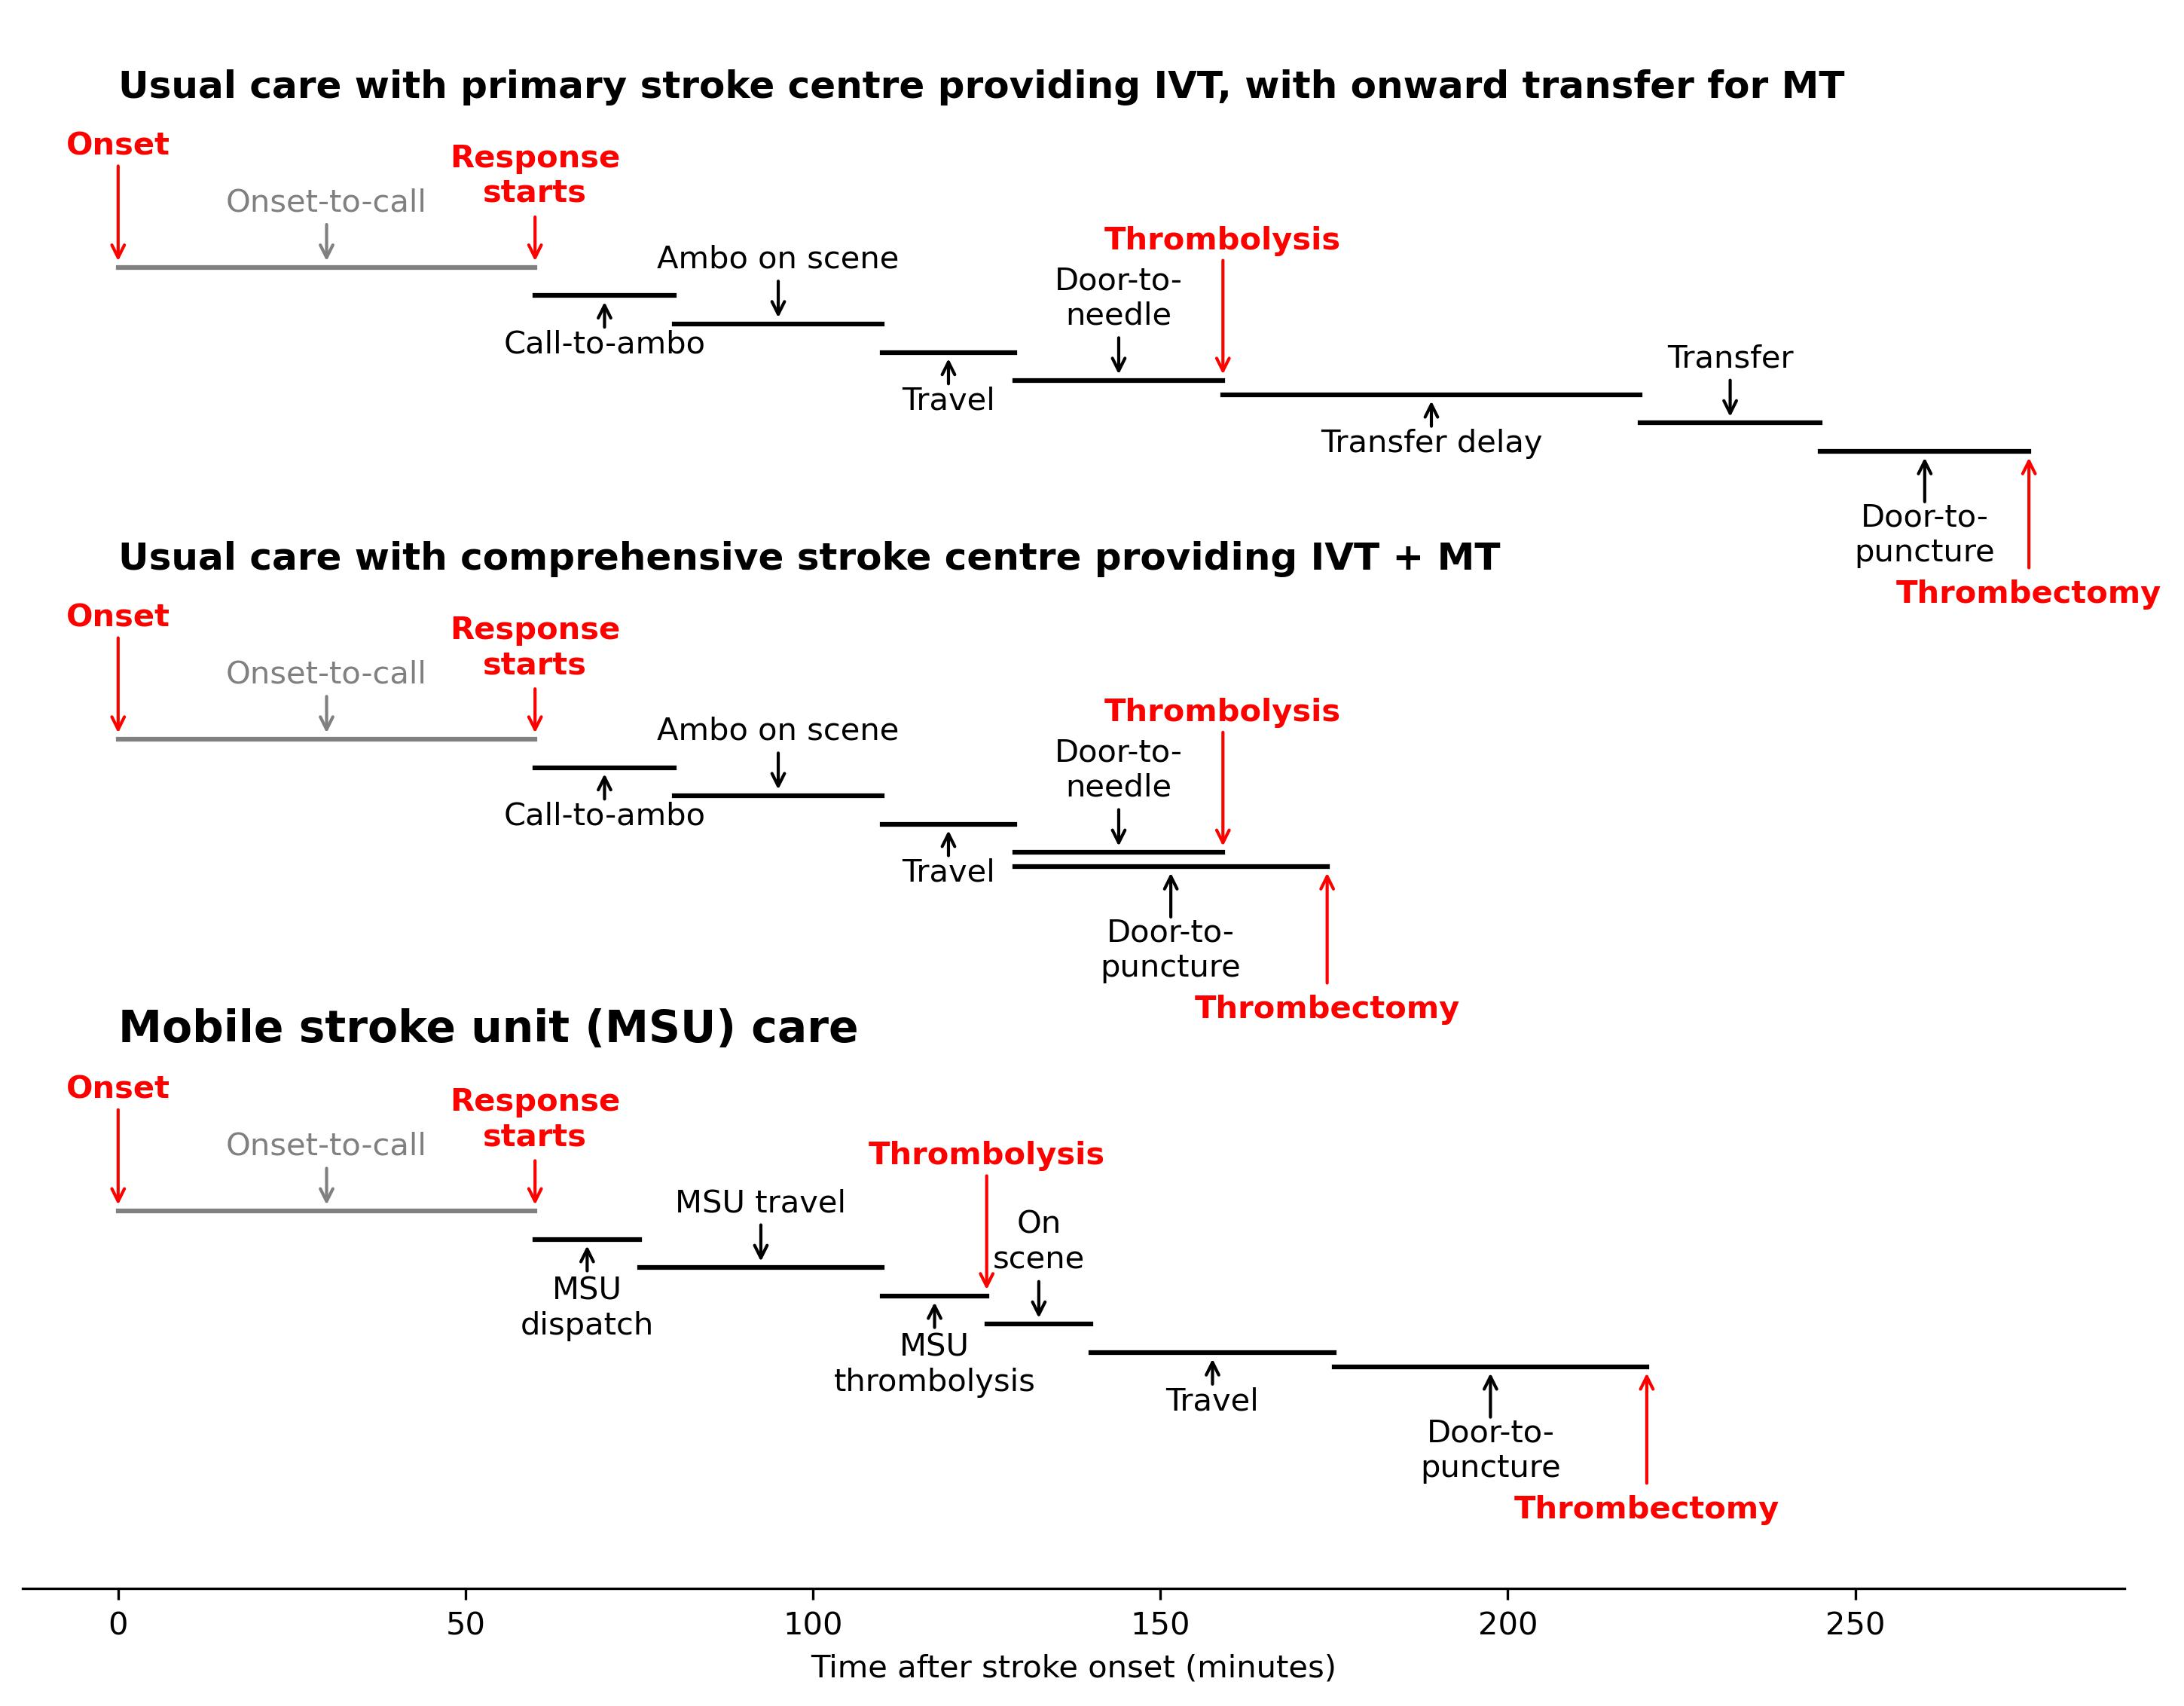
\includegraphics[width=0.85\linewidth]{images/stroke_treatment.jpg}
    \caption{Processes modeled for provision of IVT and MT. Top: First admission to a primary stroke centre providing IVT, followed by transfer to a comprehensive stroke centre for MT. Middle first admission to a comprehensive stroke centre providing both IVT and MT. Process times other than travel times are fixed for all patients. Travel times depend on locations of patient and hospitals, with results calculated for all LSOAs in England.}
    \label{fig:process}
\end{figure}

For each LSOA times to thrombolysis and thrombectomy are calculated by summing all the non-travel process times (constant for all patients) and adding required travel times (bespoke for each LSOA location, and for each inter-hospital transfer). Outcomes are then calculated based on these LSOA-specific timers to IVT and MT for usual-care or care with mobile stroke unit. All calculations are performed in Python/NumPy.


\subsection{Scenario analysis}

Scenario analysis was undertaken to investigate how changing assumed model parameters affect outcomes across all LSOAs. Parameter values were varied according to the following (all times in minutes), with all combinations modelled:

\begin{minipage}{1.0\textwidth}  % Define the width of the minipage
\begin{spacing}{1.2}
\begin{itemize}
    \item All patients:
    \begin{itemize}
        \item Stroke onset to call: 0, 60, 120, 180
    \end{itemize}
    \item Usual care:
    \begin{itemize}
        \item Call to ambulance arrival: 15, 30, 45
        \item Ambulance on-scene: 20, 30, 45
        \item Hospital arrival to IVT: 30, 45
        \item Transfer-related delay (excluding travel time): 30, 60, 90
        \item Hospital arrival to MT: 60, 90, 120
    \end{itemize}
    \item Mobile stroke units:
    \begin{itemize}
        \item Call to MSU dispatch: 0, 15, 30, 45
        \item MSU arrival to IVT: 15, 30, 45
        \item MSU on-scene post-IVT: 5, 15
        \item MSU hospital arrival to MT: 30, 60, 90
    \end{itemize}
\end{itemize}
\end{spacing}
\end{minipage}


\subsection{Geographic analysis}

To study geographic variation in benefit of MSUs, a single set of parameters was chosen, reflecting a reasonable base case for performance of normal care and MSU care. Process times (minutes) are shown below, with ambulance and MSU travel times and inter-hospital travel times dependent on patient location (LSOA). In this base case scenario MSUs are based at comprehensive stroke centres only. Admission numbers per LSOA were taken from HES 2017-2019 (using OCD-10 codes of I61, I63 and I64). Population density was taken from the Office of National Statistics 2011 census.


\begin{minipage}{1.0\textwidth}  % Define the width of the minipage
\begin{spacing}{1.2}
\begin{itemize}
    \item All patients:
    \begin{itemize}
        \item Stroke onset to call: 60
    \end{itemize}
    \item Usual care:
    \begin{itemize}
        \item Call to ambulance arrival: 20
        \item Ambulance on-scene: 30
        \item Hospital arrival to IVT: 45
        \item Transfer-related delay (excluding travel time): 60
        \item Hospital arrival to MT: 90
    \end{itemize}
    \item Mobile stroke units:
    \begin{itemize}
        \item Call to MSU dispatch: 15
        \item MSU arrival to IVT: 30
        \item MSU on-scene post-IVT: 5
        \item MSU hospital arrival to MT: 60
    \end{itemize}
\end{itemize}
\end{spacing}
\end{minipage}


\subsection{Varying number of MSU locations}

In order to study the effect of changing the number of MSU base locations, a greedy algorithm was used. In this method, 100 MSU locations are added, chosen from either only comprehensive stroke centres, or from any stroke unit type, in the order of maximum improvement in outcomes (utility). The utility gain is calculated for those patients treated by a MSU rather than usual care; the algorithm is therefore looking at the effect of changing MSU locations rather than the number of physical MSUs.